
%(BEGIN_QUESTION)
% Copyright 2015, Tony R. Kuphaldt, released under the Creative Commons Attribution License (v 1.0)
% This means you may do almost anything with this work of mine, so long as you give me proper credit

Suppose we have a Koyo ``CLICK'' PLC controlling an AC induction motor though a contactor.  The motor's 480 VAC three-phase wiring and the power sources have been eliminated from this diagram for simplicity:

$$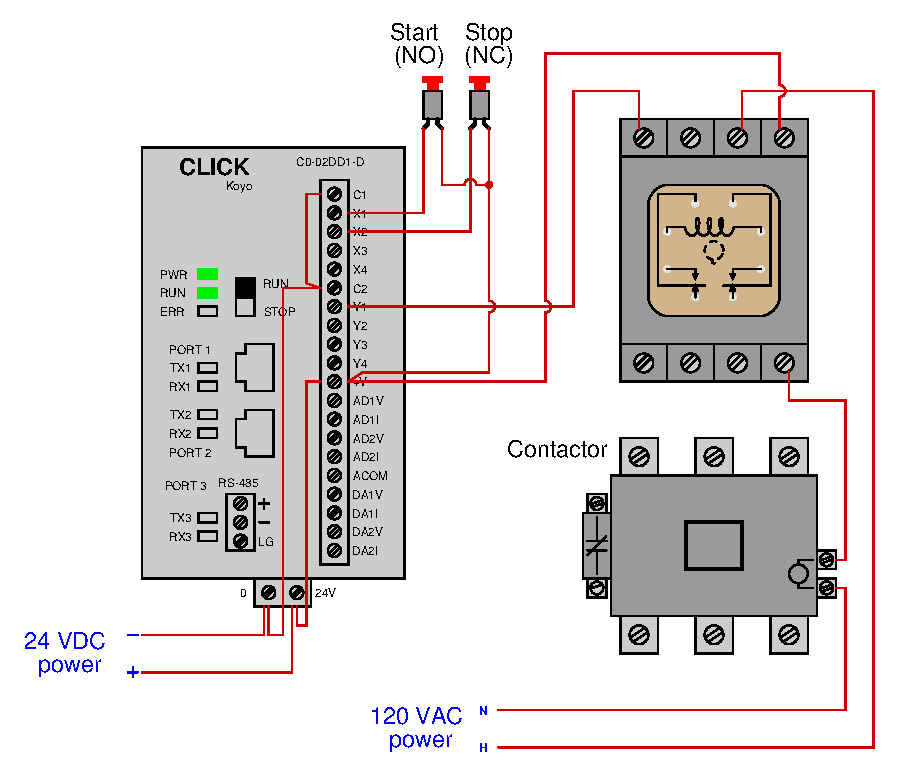
\includegraphics[width=15.5cm]{i02268x01.eps}$$

Unfortunately, the motor is not starting up when it should.  You are summoned to investigate, so you connect a laptop PC to the PLC to examine the ``live'' status of the program elements:

$$\includegraphics[width=15.5cm]{i02268x02.eps}$$

Based on your examination of this program, identify some likely faults to explain why the motor is not starting, and describe your next diagnostic step(s) in isolating the exact nature and location of the problem.  Also, determine whether the {\tt Y1} output is {\it sourcing} or {\it sinking} current.

\underbar{file i02268}
%(END_QUESTION)





%(BEGIN_ANSWER)


%(END_ANSWER)





%(BEGIN_NOTES)

The problem is in the {\it output} portion of the circuit.  Possible faults include:

\begin{itemize}
\item{} PLC's output channel failed open (not turning on)
\item{} Output wiring fault (e.g. open) anywhere in output circuit
\item{} Failed-open relay coil
\item{} Failed-open relay contact
\item{} Failed-open contactor coil
\item{} Failed-shorted contactor coil
\item{} Failed-open contactor power contact(s)
\end{itemize}

The output of this PLC is {\it sinking} current from the relay coil.

\vskip 10pt

Here, an interposing relay allows the DC sinking output of the PLC to control 120 VAC power to the contactor coil.



\vskip 20pt \vbox{\hrule \hbox{\strut \vrule{} {\bf Virtual Troubleshooting} \vrule} \hrule}

This question is a good candidate for a ``Virtual Troubleshooting'' exercise.  Presenting the diagram to students, you first imagine in your own mind a particular fault in the system.  Then, you present one or more symptoms of that fault (something noticeable by an operator or other user of the system).  Students then propose various diagnostic tests to perform on this system to identify the nature and location of the fault, as though they were technicians trying to troubleshoot the problem.  Your job is to tell them what the result(s) would be for each of the proposed diagnostic tests, documenting those results where all the students can see.

During and after the exercise, it is good to ask students follow-up questions such as:

\begin{itemize}
\item{} What does the result of the last diagnostic test tell you about the fault?
\item{} Suppose the results of the last diagnostic test were different.  What then would that result tell you about the fault?
\item{} Is the last diagnostic test the best one we could do?
\item{} What would be the ideal order of tests, to diagnose the problem in as few steps as possible?
\end{itemize}

%INDEX% PLC, relating I/O status to virtual elements

%(END_NOTES)


